\section{Descente de gradient}

La Descente de Gradient est un algorithme permettant de trouver un minimum local d'une fonction en convergeant. Elle est utilisée pour trouver le minimum d'une fonction "coût", évaluant l'erreur entre la valeur de sortie du réseau de neurones et celle attendue: \\
\begin{center}
    $f : s \mapsto (s - s_{attendue})^2$\\
\end{center}
- $s$ la sortie donnée par le modèle \\
- $s_{attendue}$ la sortie cible. \\

\subsection*{Mise en oeuvre de l'algorithme}
$f$ la fonction coût. \\
Soit $x_0$ une valeur initiale aléatoire, $t$ le taux d'apprentissage.
Supposons $x_0, \ldots, x_k$ construits. \\
• Si $\norme{\nabla f(x_k)} \leq \varepsilon$, on s'arrête. \\
• Sinon on pose $x_{k+1} = x_k - t \nabla f(x_k)$ \\

\begin{figure}[htbp!]
    \centering
    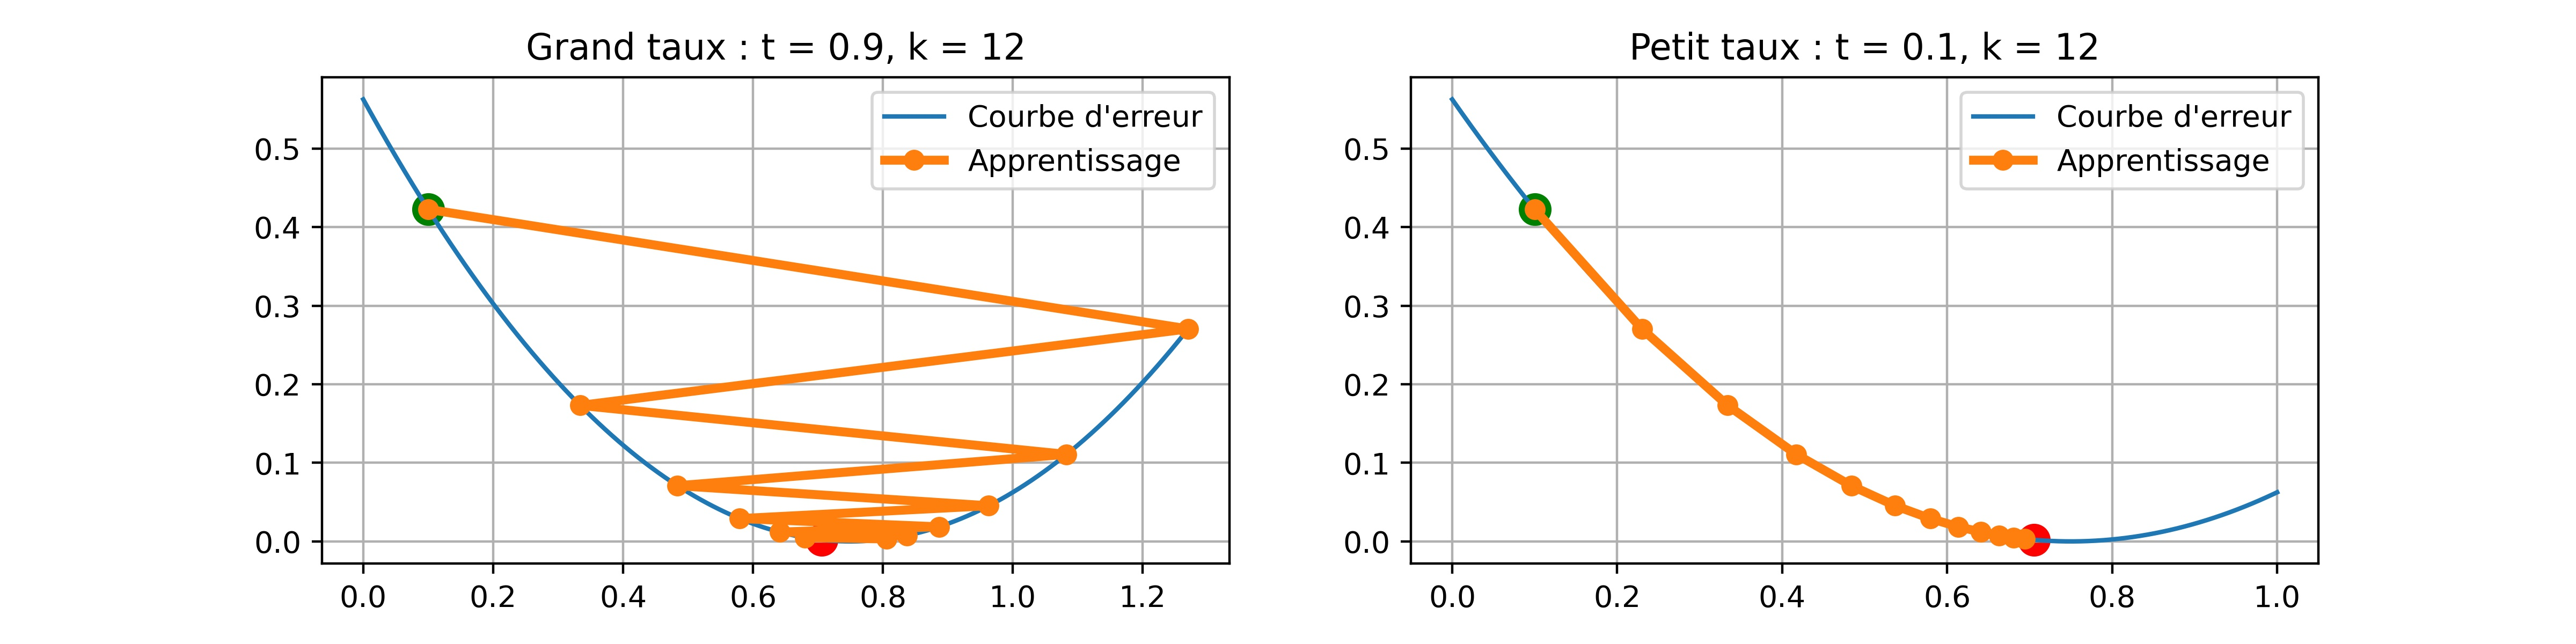
\includegraphics[width=\textwidth]{1-DescenteGradient.jpg}
    \caption{Descente de Gradient pour $f(x) = (x-0.75)^2$; $x_0=0.1$ et $\varepsilon = 0.1$}
\end{figure}

\subsection*{Importance du taux d'apprentissage}
On remarque que le choix du taux d'apprentissage à un grand impact sur l'apprentissage. Les problèmes rencontrés en fonction du choix du taux d'apprentissage : \\
- trop grand, la descente de gradient diverge \\
- trop petit , la descente de gradient converge lentement \\

$x_0$ aléatoire, momentum $\omega_0 = 0$.
        Supposons $x_0, \ldots, x_k$ et $\omega_0, \ldots, \omega_k$ construits. \\
        • On pose $\omega_{k+1} = \gamma \omega_k + t \nabla f(x_k)$ \\
        • On pose $x_{k+1} = x_k - \omega_{k+1}$